\documentclass{article}
\usepackage{CJKutf8}
\usepackage{amsmath}
\usepackage{listings}
\usepackage{graphicx}

\usepackage[a4paper, total={6in, 10.5in}]{geometry}

\title{醉酒程式-大三大四 PC}
\date{May 5, 2023}
\begin{document}
\begin{CJK*}{UTF8}{bsmi}

\maketitle

\section*{工具鯨魚}

你知道嗎,公鯨魚的個頭很大,母鯨魚的個頭很小,當公鯨魚和母鯨魚好蒿爽爽的時候是很不方便,需要另外一隻公鯨魚在下面撐著母鯨魚,不讓母鯨魚掉下來,
這樣才能完成好蒿爽爽過程。

\begin{figure*}[htb]
    \vspace{-\baselineskip}  
    \begin{center}
        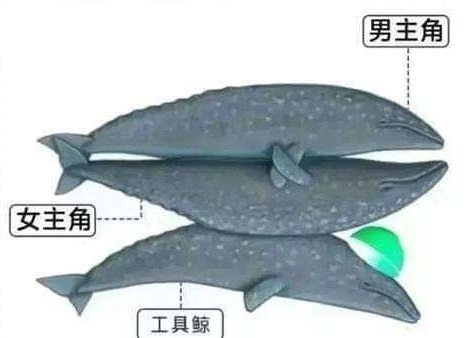
\includegraphics[scale=0.5]{whale-example.jpg}
      \caption{example}
      \label{fig:example}
    \end{center}
    \vspace{-\baselineskip}
\end{figure*}

現在假設你有一個魚缸,裡面有很多鯨魚,突然某一天他們都很想繁衍後代,所以他們疊在了一起形成一個鯨魚柱,但是你觀察到有些是公的疊在公的上?
你很想假設鯨魚也有非二元性別,但是與其做這種假設,還不如假設他們只是疊錯了,突然你想知道他們這樣到底有幾隻在好蒿爽爽,有幾隻在當工具鯨。
假設M代表公鯨、F代表母鯨,現在給你$n$個M或F字元,請找出有哪幾隻在好蒿爽爽、有哪幾隻在當工具鯨。
越前面的字元代表越上面。

注意鯨魚可以在好蒿爽爽的同時,當工具鯨魚,例如: MFMFM,有4隻在好蒿爽爽(第一、二隻,第三、四隻),而同時也有2隻在當工具鯨魚(第三、五隻)

\begin{figure*}[htb]
    \vspace{-\baselineskip}  
    \begin{center}
        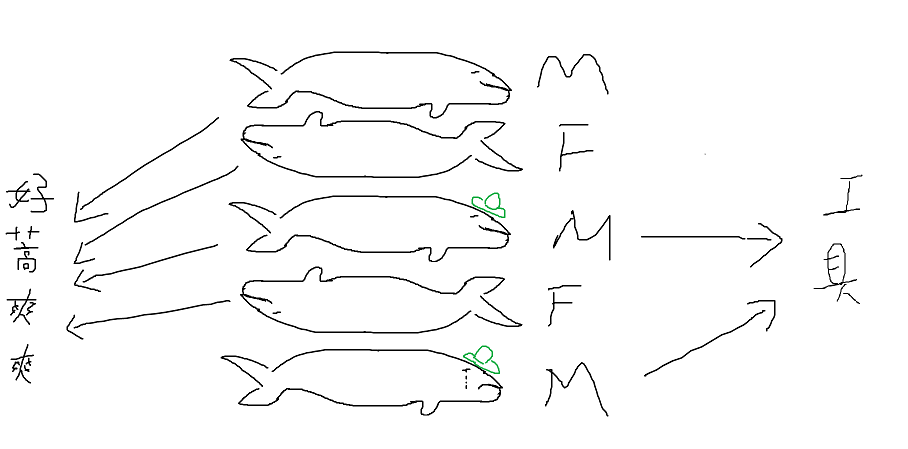
\includegraphics[scale=0.6]{whale-example2.png}
      \caption{example2}
      \label{fig:example2}
    \end{center}
    \vspace{-\baselineskip}
\end{figure*}

\subsection*{輸入格式}
第一行有一個數字$n$,代表接下來有$n$個字元。
第二行有一個$n$個M或F組成的字串。

\subsection*{輸出格式}
輸出有幾隻在好蒿爽爽,有哪些在當工具鯨魚,以空白分隔。

\subsection*{輸入範例}
$13\\\text{FMMFMMFFMMFFF}$

\subsection*{輸出範例}
2 1

\subsection*{測資範圍}
\begin{itemize}
    \item testcase 1-2, $n=5$, 占分: $20\%$
    \item testcase 3-5, $n=10$, 占分: $30\%$
    \item testcase 6-7, $n=100$, 占分: $20\%$
    \item testcase 8-10, $n=10^6$, 占分: $30\%$
\end{itemize}

\end{CJK*}
\end{document}